\pagestyle{VS}
\chapter{Crisi della fisica classica}
Argomento di studio di questo caso è \textbf{la meccanica quantistica}. La meccanica quantistica descrive \textbf{la materia e la luce (radiazione) in tutti i suoi aspetti, in particolare per quanto riguarda i fenomeni microscopici}, che avvengono cioè su scala atomica.\\

La meccanica quantistica, dunque, sostituisce le leggi della fisica ``classica'' (meccanica ed elettromagnetismo) nella descrizione più accurata della materia. Manifestandosi principalmente nel comportamento di sistemi microscopici, la meccanica quantistica \textbf{descrive fenomeni completamente diversi da quelli ai quali ci ha abituato l'esperienza}. In questo risiede la principale \textbf{difficoltà} che incontriamo nel ``capire'' la meccanica quantistica. Formalmente la matematica che entra nella formulazione delle leggi quantistiche non è più complessa di quella richiesta dalle leggi classiche (è la matematica delle onde e degli spazi vettoriali complessi).\\

Lo sviluppo della meccanica quantistica ha rappresentato, insieme a quello della teoria della relatività, una \textbf{rivoluzione scientifica} nel ventesimo secolo. Per quanto riguarda la meccanica quantistica, questo è dovuto non solo all'introduzione di leggi nuove ma anche e soprattutto al carattere di queste nuove leggi. In particolare, \textbf{le leggi quantistiche non sono deterministiche nel senso classico}. Non possono prevedere gli eventi che occorreranno nell'evoluzione di un sistema fisico, ma solo le \textbf{le probabilità} con cui diversi eventi potranno occorrere. E questa caratteristica non è determinata da una nostra conoscenza incompleta del sistema fisico (come nel lancio di un dado) o della teoria stessa, ma è intrinseca nel mondo fisico. \textbf{Non esistono ``variabili nascoste''}, come diversi fisici hanno per lungo tempo ipotizzato.\\

Per illustrare meglio il percorso che ha condotto allo sviluppo della meccanica quantistica ricordiamo sommariamente \textbf{qual era la fisica} classica, ossia la fisica conosciuta \textbf{prima del '900}.  A quell'epoca i fisici ritenevano di avere oramai compreso le leggi fondamentali in grado di spiegare, almeno in principio, qualunque fenomeno fisico.\\

Nel \textbf{1600} si era giunti, grazie in particolare all'opera di \textbf{Newton}, alla formulazione completa delle \textbf{leggi del moto} (meccanica). In particolare la seconda legge del moto, $F=ma$, è un'equazione che può essere ``integrata'': note le posizioni e le velocità iniziali delle parti che costituiscono un sistema, è possibile determinare con esattezza le posizioni e le velocità di queste parti ad un qualunque istante di tempo successivo. In questa possibilità risiede il \textbf{carattere deterministico della meccanica classica}. Nota l'equazione del moto, compito della fisica diventa lo studio delle \textbf{forze}. Lo stesso Newton comprende la \textbf{gravitazione} e formula la sua legge di gravitazione universale.\\

Lo studio dei \textbf{fenomeni elettrici e magnetici} conduce ad una loro descrizione esaustiva nella seconda metà dell'800, con la formulazione delle \textbf{equazioni di Maxwell}. Queste evidenziano la completa unificazione dei fenomeni elettrici e magnetici, che sono diversi aspetti dello stesso fenomeno e che si evidenziano a seconda del sistema di riferimento dal quale vengono osservati.\\

Le equazioni di Maxwell mostrano inoltre come i campi elettrico e magnetico si propagano tramite \textbf{onde elettromagnetiche}, di cui la \textbf{luce} (visibile) non è che un esempio in un particolare intervallo di lunghezze d'onda. Questo risultato sembrava porre fine alla antica diatriba circa la \textbf{natura corpuscolare od ondulatoria della luce}. La prima, sostenuta dallo stesso Newton, era stata messa fortemente in crisi dall'osservazione, in particolare nel corso del 1700, dai fenomeni prettamente ondulatori quali l'interferenza e la diffrazione della luce. La risposta, apparentemente definitiva, fornita dalla teoria di Maxwell era destinata tuttavia ad essere messa nuovamente in discussione nei primi anni del '900.\\

Più in generale, nel periodo che va dalla fine del diciannovesimo secolo ai primi anni del ventesimo secolo, una serie di risultati sperimentali, riguardanti fenomeni che avvengono su scala atomica, hanno portato ad una \textbf{crisi della fisica classica}. L'interpretazione di questi risultati ha richiesto un cambiamento radicale nelle concezioni e nelle leggi classiche fondamentali, ed ha portato allo sviluppo della meccanica quantistica. Discutiamo di seguito alcuni di questi risultati che hanno evidenziato, in particolare, le \textbf{proprietà corpuscolari della radiazione} e , per contro, \textbf{proprietà ondulatorie della materia}.

\section{Lo spettro di corpo nero}
Tutti i corpi, investiti da una radiazione elettromagnetica, trasmettono, riflettono o assorbono la radiazione incidente. Un \textbf{corpo nero} è un corpo che \textbf{assorbe completamente la radiazione incidente}. I corpi, se riscaldati ad una certa temperatura, emettono anche radiazione (es: mano vicina ad un ferro da stiro caldo).\\

Indichiamo con $E(\omega , T) $ il \textbf{potere emissivo} di un corpo, ossia la quantità di energia emessa per unità di volume dal corpo, mediante radiazione di frequenza $\omega$, quando questo viene riscaldato alla temperatura $T$. Analogamente indichiamo con $A(\omega , T )$ il \textbf{potere assorbitivo}, ossia la frazione di energia che viene assorbita da un corpo, rispetto a quella totale incidente, quando questo viene investito da una radiazione di frequenza $\omega$ e si trova in equilibrio termico alla temperatura  $T$.
Era stato osservato da \textbf{Kirchoff}, nell'800, che il rapporto tra il potere emissivo e potere assorbitivo di un corpo è una funzione universale, ossia indipendente dal corpo:
	\begin{equation}
		\tcboxmath[sharp corners=downhill ,colback=white,colframe=red!75!black]{
			\frac{E(\omega ,T)}{A(\omega ,T)}= u(\omega , T),
		}
	\end{equation}
detta \textbf{Legge di Kirchoff}, con $u(\omega , T)$ funzione universale.\\

Per un corpo nero il potere assorbitivo è uguale ad uno, indipendentemente dalla frequenza e dalla temperatura. La funzione universale coincide pertanto con il potere emissivo del corpo nero:
	\begin{equation}
		u(\omega, T)= E(\omega , T)|_{corpo\ nero}.
	\end{equation}\\
	
Il potere emissivo del corpo nero coincide anche con la distribuzione della densità di energia della \textbf{radiazione e.m. in equilibrio termico all'interno di una cavità} a temperatura $T$. Se immaginiamo di praticare un piccolo foro nella cavità, questa si comporta come un ``corpo nero'': assorbe la radiazione incidente su tutte le frequenze, perché un raggio che entra non può più uscire:\\
	\begin{figure}[!htbp]
		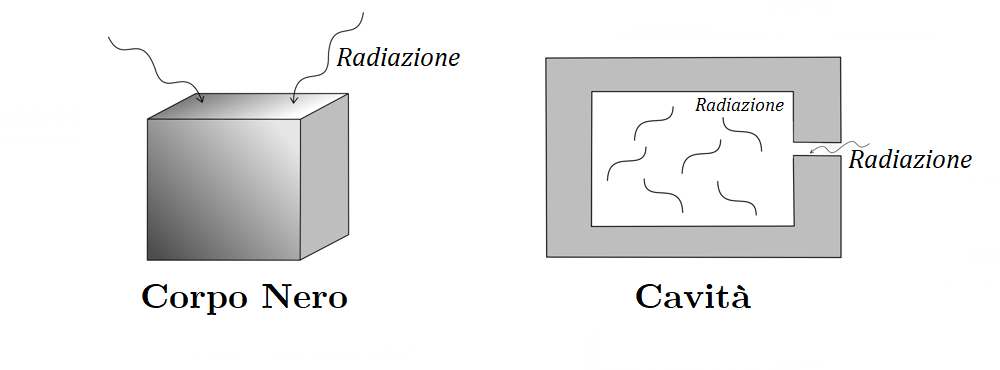
\includegraphics[width=\textwidth]{immagini/cap_1/fig_1_1.png}
	\end{figure}
	
Il problema nello studio del potere emissivo del corpo nero era rappresentato dalla \textbf{discrepanza tra le osservazioni sperimentali e la descrizione teorica}.
	\begin{figure}[!htbp]
		\begin{center}
			\includegraphics[width=.7\textwidth]{immagini/cap_1/fig_1_2.png}
		\end{center}
	\end{figure}
	
La descrizione teorica dello spettro di energia del corpo nero riguardava due regioni: \textbf{a basse frequenze} risultava valida la previsione della fisica classica, espressa dalla cosiddetta \textbf{formula di Rayleigh-Jeans}:
	\begin{equation}
		\tcboxmath[sharp corners=downhill ,colback=white,colframe=red!75!black]{
			u(\omega , T)= \frac{\omega ^2}{\pi ^2 c^3}KT,
		}
			\qquad \textrm{ \footnotesize{(piccoli $\omega$)} }
	\end{equation}
dove $K$ è la costante di Boltzmann e c la velocità della luce. Ad alte frequenze risultava invece valida una formula empirica, senza alcuna interpretazione teorica, detta \textbf{formula di Wien}:
	\begin{equation}
		\tcboxmath[sharp corners=downhill ,colback=white,colframe=red!75!black]{
			u(\omega ,T)= C \omega ^3 e^{-\lambda \omega /T},
		}
			\qquad \textrm{\footnotesize{(grandi $\omega$)}}
	\end{equation}
con $C$ e $\lambda$ costanti. Come è mostrato in figura, né la formula classica, né  la formula empirica di Wien descrivevano la distribuzione spettrale nella regione di frequenze intermedie.
Nel \textbf{1900, Max Planck} derivò la sua famosa formula per lo spettro di corpo nero mediante un'ingegnosa interpolazione tra la formula di Rayleigh-Jeans e la formula di Wien. La \textbf{formula}, suggerita da\textbf{Planck},
	\begin{equation}
	\tcboxmath[enhanced,sharp corners=downhill ,colback=yellow!50!white,colframe=red!75!black, borderline={2pt}{-3pt}{red!50!black}]{
		u(\omega, T) = \frac{\hbar}{\pi ^2 c^3}\frac{\omega ^3}{e^{\hbar \omega / KT}-1},
	}
\end{equation}
risultava in perfetto accordo con le misure sperimentali. Il valore ottenuto per la \textbf{``costante di Planck''} è
\[ \tcboxmath[sharp corners=downhill ,colback=white,colframe=red!75!black]{\hbar = 1.054 \cdot 10^{-27} \ erg\cdot s.}\]
Questa costante giocherà un ruolo fondamentale nella meccanica quantistica.\\

È immediato verificare come nei limiti di basse ed alte frequenze la formula di Planck riproduce correttamente gli andamenti già noti:\\
\begin{equation}
u(\omega , T) =\frac{\hbar}{\pi ^2 c^2} \frac{\omega ^3}{e^{\frac{\hbar \omega}{KT}} -1} 
\begin{array}{clcc}
 & \displaystyle{\frac{\omega ^2}{\pi ^2 c^3} } & \textrm{per } \hbar \omega \ll KT, & \textrm{[Rayleigh-Jeans]}\\
\nearrow \\
\searrow \\
 & \displaystyle{\frac{h}{\pi ^2 c^3}\omega ^3 e^{\frac{-\hbar \omega}{KT}}} & \textrm{per }  \hbar \omega \gg KT .& \textrm{[Wien]}
\end{array}
\end{equation}

Il perfetto accordo della sua formula indusse Planck a cercare una \textbf{spiegazione teorica}. Per comprendere la spiegazione trovata da Planck è utile discutere prima la derivazione della formula di Rayleigh-Jeans ottenuta utilizzando le leggi della fisica classica. Osserviamo anche che la formula di  Rayleigh-Jeans non poteva comunque, in generale, essere corretta perché conduce ad una densità di energia totale (integrata su tutte le frequenze) infinita (``catastrofe ultravioletta''):
	\begin{equation}
		E(T) = \int _0 ^\infty d\omega\ u(\omega , T) \overset{R.J.}{=} \frac{KT}{\pi ^2 c ^3}\int _0 ^\infty d\omega \ \omega ^2 = \infty \textrm{(!)}
	\end{equation}
La formula classica di Rayleigh-Jeans era derivata calcolando il numero di modi normali di oscillazione della radiazione elettromagnetica con frequenza compresa tra $\omega$ ed $\omega + d\omega$ ed associando a ciascun modo un'energia media $KT$ (in accordo con la legge classica di equipartizione dell'energia). Discutiamo la derivazione di entrambi questi risultati.\\
Calcoliamo il numero di modi normali di oscillazione della radiazione elettromagnetica con frequenza compresa tra $\omega$ ed $\omega + d\omega$. \\
Un'onda che si propaga nella direzione $x$ con vettore d'onda $k_x$, è descritta dalla funzione $e^{ik_x x}$. Se consideriamo per il campo e.m. nella cavità con volume finito condizioni al bordo periodiche, allora il vettore d'onda $k_x$ è soggetto alla condizione:
	\begin{eqnarray}
		e^{ik_x x}= e^{ik_x (x+L)} \Rightarrow e^{ik_x L}=1  \nonumber\\ \Rightarrow k_x=\frac{2\pi}{L}n, \qquad n= 0, \pm 1, \pm 2,...
	\end{eqnarray}
dove $L$ è la lunghezza del volume nella direzione $x$. Il numero $dn_x$ di modi normali di oscillazione con vettore d'onda $k_x$ compreso tra $k_x$ e $k_x+dk_x$ è allora:
	\begin{equation}
		dn_x =\frac{L}{2\pi}dk_x.
	\end{equation}
Considerando le 3 direzioni spaziali del vettore d'onda ed i fatto che per ciascun' onda di vettore $\vec{k}$ esistono 2 gradi di polarizzazione indipendenti otteniamo per il numero totale di oscillazioni con frequenza compresa tra $\omega$ e $\omega + d\omega$ il valore
	\begin{equation}
		dn =2\frac{V}{(2\pi)^3}d^3k= V \frac{2\cdot 4\pi}{8\pi ^3} k^2 dk \overset{\omega =ck}{=} V \left( \frac{\omega ^2}{\pi ^2 c^3}\right) d\omega .
	\end{equation}
Il primo fattore che entra nella formula di Rayleigh-Jeans,
	\begin{equation}
		\tcboxmath[sharp corners=downhill ,colback=white,colframe=red!75!black]{
			\left( \frac{\omega ^2}{\pi ^2 c^3} \right) ,
		}
		\label{eq:cap1_1}
	\end{equation}
rappresenta dunque il \textbf{numero di modi normali di oscillazione della radiazione, per unità di volume, con frequenza compresa tra $\omega$ e $\omega + d\omega$}.\\

Dimostriamo ora come il secondo fattore, $KT$, rappresenti secondo la fisica classica l'energia media di ciascun oscillatore armonico. A tale scopo è necessario introdurre alcuni concetti di \textbf{meccanica statistica}.\\
Secondo la meccanica statistica, la probabilità che un sistema mantenuto in equilibrio in equilibrio termico alla temperatura $T$ si trovi in uno stato $s$ corrispondente ad un'energia $E_s$ è data da:
	\begin{equation}
		p(E_s) =\frac{1}{Z}e^{\frac{-E_s}{KT}},
	\end{equation}
dove $Z$, detta funzione di partizione, è l'opportuna costante di normalizzazione della probabilità:
	\begin{equation}
		Z= \sum _s e^{-E_s / KT}.
	\end{equation} 
La sommatoria su $s$ è estesa qui a tutti i possibili stati microscopici del sistema.\\
Da quanto detto segue anche che l'energia media del sistema, mantenuto in equilibrio alla temperatura $T$, è data da:
	\begin{equation}
	\langle E \rangle = \sum _s p(E_s)\cdot E_s = \frac{1}{Z}\sum _s E_s e^{-\frac{E_s}{KT}}.
	\end{equation}

Applichiamo questi ora questi concetti per calcolare l'energia media di un oscillatore armonico unidimensionale in equilibrio alla temperatura $T$. La Hamiltioniana dell'oscillatore è:
	\begin{equation}
		H= \frac{p^2}{2m}+\frac{1}{2}m \omega ^2 x^2 , 
	\end{equation}
e la ``somma sugli stati'' dell'oscillatore è un integrale su tutti i possibili valori di impulso e posizione:
	\begin{equation}
		\sum _s = \iint dp dx .
	\end{equation}
L'energia media dell'oscillatore è allora: ($\beta = 1/KT$)
	\begin{eqnarray}
		\langle E \rangle &=& \frac{\int _{-\infty} ^{+\infty} dp\ dx \ e^{-\beta \left( \frac{p^2}{2m}+\frac{1}{2}m \omega ^2x^2\right)}\left( \frac{p^2}{2m}+\frac{1}{2}m \omega ^2x^2\right)}{\int _{-\infty} ^{+\infty} dp\ dx\ e^{-\beta \left( \frac{p^2}{2m}+\frac{1}{2}m \omega ^2x^2\right)}}= \nonumber \\
		&=&\frac{\int _{-\infty} ^{+\infty} dp \ e^{-\beta \left( \frac{p^2}{2m}\right)}\left( \frac{p^2}{2m}\right)}{\int _{-\infty} ^{+\infty} dp \  e^{-\beta \left( \frac{p^2}{2m}\right)}} + \frac{\int _{-\infty} ^{+\infty}  dx \  e^{-\beta \left(\frac{1}{2}m \omega ^2x^2\right)}\left(\frac{1}{2}m \omega ^2x^2\right)}{\int _{-\infty} ^{+\infty} dx\ e^{-\beta \left( \frac{1}{2}m \omega ^2x^2\right)}}= \nonumber \\
		&=& 2\cdot \frac{\int _{-\infty} ^{+\infty}ds \  e^{-\beta s^2}s^2}{\int _{-\infty} ^{+\infty}ds \  e^{-\beta s^2}}= \qquad \scriptstyle{\textrm{N.B. } s=\frac{p}{\sqrt{2m}}, \ s= \sqrt{\frac{m \omega ^2}{2}}x}\nonumber \\
		&=&-2 \frac{\partial}{\partial \beta} \ln \left(\int _{-\infty} ^{+\infty}ds \  e^{-\beta s^2} \right) = -2\frac{\partial}{\partial \beta} \ln \sqrt{\frac{\pi}{\beta}}= \nonumber \\
	&=& \frac{\partial}{\partial \beta} \ln \beta = \frac{1}{\beta}= KT. 
	\end{eqnarray}
Troviamo dunque il risultato cercato:
	\begin{equation}
	\tcboxmath[sharp corners=downhill ,colback=white,colframe=red!75!black]{
			\langle E \rangle = KT.
	}
	\label{eq:cap1_2}
\end{equation}
Moltiplicando questa energia media di ciascun oscillatore per il numero di oscillatori (eq. (\ref{eq:cap1_1})) si ottiene la formula di Rayleigh-Jeans.\\

Planck trovò che la sua formula  per lo spettro di corpo nero poteva essere derivata assumendo che l'energia associata con ciascun modo del campo elettromagnetico non può variare con continuità, come predetto dalla fisica classica, ($E= p^2/2m +1/2 \ m \omega ^2 x^2$), ma deve essere un multiplo intero di un \textbf{``quanto''} minimo di energia $\varepsilon$, legato alla frequenza $\omega$ del modo normale da:
	\begin{equation}
		\tcboxmath[enhanced,sharp corners=downhill ,colback=yellow!50!white,colframe=red!75!black, borderline={2pt}{-3pt}{red!50!black}]{
			\varepsilon = \hbar \omega .
			}
	\end{equation}
L'energia ha dunque forma:
	\begin{equation}
	\tcboxmath[enhanced,sharp corners=downhill ,colback=yellow!50!white,colframe=red!75!black, borderline={2pt}{-3pt}{red!50!black}]{
		E_n = n\varepsilon = n \hbar \omega \quad n= 0,1,2...
		}
\end{equation}
In questo caso infatti, l'energia media associata a ciascun modo normale a temperatura $T$ è data da:
	\begin{eqnarray}
		\langle E \rangle &=&\sum _n p(E_n) E_n =\frac{1}{Z}\sum _n ^{\infty} e^{-\beta n \hbar \omega} \cdot n\hbar \omega = \nonumber \\
		&=&\frac{\sum _n ^{\infty} e^{-\beta n \hbar \omega} \cdot n\hbar \omega}{\sum _n ^{\infty} e^{-\beta n \hbar \omega}}= - \frac{\partial}{\partial \beta} \ln \left( \sum _n ^{\infty} e^{-\beta n \hbar \omega}\right)= \nonumber \\
		&=&- \frac{\partial}{\partial \beta} \ln \left( \frac{1}{1- e^{-\beta \hbar \omega}}\right)=  \frac{e^{-\beta \hbar \omega}\ \hbar \omega}{1-e^{-\beta \hbar \omega}}= \frac{ \hbar \omega}{e^{\beta \hbar \omega}-1},
	\end{eqnarray}
ossia
	\begin{equation}
		\tcboxmath[enhanced,sharp corners=downhill ,colback=yellow!50!white,colframe=red!75!black, borderline={2pt}{-3pt}{red!50!black}]{
			\langle E \rangle = \frac{ \hbar \omega}{e^{\beta \hbar \omega}-1}.
			}
	\end{equation}
Questa energia, moltiplicata per il numero di modi normali per unità di volume con frequenza compresa tra $\omega$ ed $\omega + d\omega$, fornito dalla formula (\ref{eq:cap1_1}), conduce alla formula di Planck.\\

Lo spettro di corpo nero sembrava dunque indicare che la \textbf{la radiazione elettromagnetica si comporta come se fosse costituita da un insieme di quanti di energia con energia pari ad $\hbar \omega $.}
L'origine di questo comportamento risultava però ancora oscuro. Il passo successivo, che contribuì a chiarire la conclusione di Planck, si ebbe cinque anni dopo, con l'interpretazione fornita da Einstein dell'effetto fotoelettrico.
\section{L'effetto fotoelettrico}
L'effetto fotoelettrico, scoperto nel 1887 da Hertz, venne spiegato da \textbf{Einstein} nel \textbf{1905} utilizzando il concetto di natura quantistica (corpuscolare) della luce.\\
L'\textbf{effetto fotoelettrico} può essere riassunto nel modo seguente:
\begin{enumerate}
\item Quando una superficie metallica viene investita da un'onda luminosa può emettere elettroni;
\item  l'emissione o meno di elettroni dipende dalla frequenza della luce incidente. In generale esiste una \textbf{soglia} (che varia da metallo a metallo) per cui solo frequenze maggiori della soglia producono la corrente fotoelettrica;
\item l' \textbf{intensità della corrente}, quando esiste, è proporzionale all'intensità della radiazione luminosa;
\item l'\textbf{energia dei fotoelettroni} è indipendente dall'intensità della luce ma varia linearmente con la frequenza della luce incidente.
\end{enumerate} 
\textbf{Classicamente, l'effetto fotoelettrico risulta inspiegabile}. Secondo l'elettrodinamica classica, infatti, l'energia trasportata da un'onda elettromagnetica è proporzionale all'intensità dell'onda, ed indipendente dalla frequenza. Non è possibile pertanto spiegare perché l'effetto abbia una soglia dipendente dalla frequenza e perché l'energia dei fotoelettroni dipenda dalla frequenza. Per spiegare l'effetto fotoelettrico \textbf{Einstein partì dall'ipotesi che la radiazione luminosa è costituita da quanti di energia $\hbar \omega$}, dove $\omega$ è la frequenza della luce. \textbf{L'assorbimento da parte di un elettrone del metallo di un singolo quanto di luce}, o fotone, come venne in seguito chiamato, accresce l'energia dell'elettrone di una quantità $\hbar \omega$. Una parte di questa energia, $W$, detta \textbf{funzione lavoro}, deve essere spesa per separare l'elettrone dal metallo. Questa energia varia da metallo a metallo. L'energia restante è disponibile come energia cinetica dell'elettrone fotoemesso. La \textbf{conservazione dell'energia} nel processo implica pertanto la seguente relazione tra la velocità dell'elettrone $v$ e la frequenza $\omega$ della luce:
	\begin{equation}
		\tcboxmath[sharp corners=downhill ,colback=white,colframe=red!75!black]{
			\frac{1}{2}m v^2= \hbar - W.
			}
	\end{equation}
La presenza di una soglia e la relazione lineare tra energia dell'elettrone e frequenza sono contenute in questa formula.\\

La proporzionalità tra la corrente fotoelettrica ed intensità della sorgente luminosa può pure essere spiegata in termini di quanti di luce: una sorgente di luce più intensa emette più fotoni e questi, a loro volta, liberano più elettroni.\\

La correttezza della formula di Einstein venne verificata in una serie di esperimenti, in particolare da \textbf{Millikan}. L'effetto fotoelettrico venne così a costituire una delle forti evidenze sperimentali a favore della natura corpuscolare della luce.
\section{L'effetto Compton}
L'\textbf{effetto Compton} (1922) è forse il fenomeno fisico che, più di ogni altro, ha fornito un'evidenza diretta della natura corpuscolare della luce.\\

\textbf{Compton scoprì che la radiazione di una certa lunghezza d'onda} (nella regione dei raggi x) \textbf{fatta incidere su di un foglio metallico, veniva diffusa con lunghezza d'onda differente dalla lunghezza d'onda della luce incidente, e la differenza delle lunghezze d'onda dipendeva dall'angolo di diffusione}.\\

Secondo \textbf{l'elettrodinamica classica}, la diffusione della luce è dovuta all'irraggiamento da parte degli elettroni atomici, che vengono posti in oscillazioni forzate dalla luce incidente. In questo caso la lunghezza d'onda diffusa è prevista essere uguale alla lunghezza d'onda della luce incidente e l'intensità ha una dipendenza dall'angolo $\theta$ di diffusione dato da $(1+cos^2 \theta)$ (\textbf{scattering Thomson}).\\

Lo spostamento osservato nella lunghezza d'onda della luce diffusa viene spiegato da Compton considerando la radiazione incidente come fascio di fotoni di energia $\hbar \omega$. \textbf{I singoli fotoni vengono diffusi elasticamente dai singoli elettroni:}
	\begin{figure}[!htbp]
		\begin{center}
			\includegraphics[width=.6\textwidth]{immagini/cap_1/fig_1_3.png}
		\end{center}
	\end{figure}
	
	
Un fotone di frequenza $\omega$ e vettore d'onda $\vec{k}$ ha energia $E = \hbar \omega$ ed impulso $\vec{q}= \hbar \vec{k}$. La relazione relativistica $E=cq$, valida per particelle di massa nulla, implica $\omega = c|\vec{k}|$. I 4-vettori energia.impulso per il fattore incidente ed il fotone diffuso hanno dunque la forma:
	\begin{equation}
		q=\left(\frac{\bar \omega}{c}; \hbar \vec{k} \right)\qquad q' = \left(\frac{\bar \omega'}{c}; \hbar {\vec{k}}^{\, \prime}\right),
	\end{equation}
e si ha:
	\begin{equation}
		q^2 = q^{\prime \, 2}=0.
	\end{equation}
Poiché l'elettrone si trova inizialmente in quiete il suo 4-vettore energia-impulso è dato da:
	\begin{equation}
		p=\left(mc, \vec{0} \right)\qquad p^2 =m^2 c^2.
	\end{equation}
La legge di \textbf{conservazione del 4-impulso} nel processo si scrive:
	\begin{equation}
		p+q=p'+q',
	\end{equation}
da cui:
	\begin{eqnarray}
	p^{\prime \, 2} &=& m^2 c^2 = \left( p +q -q'\right)^2= p^2 + q^2 +q^{\prime \, 2}+ 2pq - 2pq' -2 qq'= \nonumber \\
	&=& m^2c^2 + 2m\hbar \omega - 2m \hbar \omega ' - 2 \frac{\hbar \ \omega \omega '}{c^2}+2 \hbar \ k k'  \cos \theta ,
	\end{eqnarray}
ossia:
	\begin{equation}
		\tcboxmath[sharp corners=downhill ,colback=white,colframe=red!75!black]{
			\omega - \omega ' =\frac{\hbar}{m c^2} \omega \omega ' \left( 1-\cos \theta \right).
			}
	\label{eq:cap1_3}
	\end{equation}
\begin{center}
\begin{tcolorbox}[toprule=3mm, width=.9\textwidth, colback=white]
\textbf{Cinematica effetto Compton}: calcolo non esplicitamente relativistico\\
	\begin{center}
	\includegraphics[width=\textwidth]{immagini/cap_1/fig_1_4.png}
	\end{center}
	\begin{equation}
		\left\{
			\begin{aligned}
			&\hbar \omega +m c^2 = \hbar \omega ' +\sqrt{m^2 c^4 + c^2 p'^2}\quad \textrm{Cons. dell'energia (1)}\\
			& \hbar \vec{k} = \hbar \vec{k'} + \vec{p'}\qquad \qquad \qquad \qquad \quad \textrm{Cons. dell'impulso (2)}
			\end{aligned}
		\right.
	\end{equation}
	\begin{eqnarray}
		c^2 p^{\prime \, 2} &\overset{\textrm{(2)}}{=}& c^2\hbar^2 \left( \vec{k}- {\vec{k}	}^{\, \prime} \right) ^2 = \hbar ^2 c^2 \left(k^2+k^{\prime \, 2}-2kk' \cos \theta \right) \nonumber \\
		&=& \hbar ^2 \left(\omega ^2 + \omega^{\prime \, 2} - 2 \omega \omega ' \cos \theta  \right)\overset{\textrm{(1)}}{=} \nonumber \\
		&=& \left( \hbar \omega - \hbar \omega ' + m c^2 \right) ^2 - m^2 c^4= \nonumber \\
		&=& {\hbar}^2 \left({\omega}^2 + {\omega}^{\prime \, 2} - 2 \omega \omega ' \right) + 2 mc^2 \hbar ( \omega - \omega ' ) \Rightarrow \nonumber \\
		&\Rightarrow & \omega - \omega' =\frac{\hbar}{m c^2} \omega \omega ' \left( 1- \cos \theta \right).
	\end{eqnarray}
\end{tcolorbox}
\end{center}

Esprimiamo questo risultato in termini delle lunghezze d'onda dei fotoni incidente e diffuso. Queste sono legate alle frequenze dalla relazione:
	\begin{equation}
		\omega = c k =\frac{2 \pi c}{\lambda} \Rightarrow \tcboxmath[sharp corners=downhill ,colback=white,colframe=red!75!black]{\lambda =\frac{2 \pi c}{\omega}.}
	\end{equation}
Moltiplicando entrambi i membri dell'equazione (\ref{eq:cap1_3}) per $2 \pi c / \omega \omega '$ si ottiene:
	\begin{equation}
		\tcboxmath[enhanced,sharp corners=downhill ,colback=yellow!50!white,colframe=red!75!black, borderline={2pt}{-3pt}{red!50!black}]{
			\lambda - \lambda ' =\frac{h}{mc}\left( 1-\cos \theta \right),
			}
	\end{equation}
che esprime lo spostamento della lunghezza d'onda del fotone diffuso, $\lambda ' $, in termini della lunghezza d'onda del fotone incidente $\lambda$. Questa previsione risultò in perfetto accordo con i dati sperimentali.\\

La quantità $\hbar/ mc$, che ha dimensioni di una lunghezza, è detta \textbf{lunghezza d'onda Compton dell'elettrone} e vale:
\[
\frac{\hbar}{mc}= 2\pi \frac{e^2}{mc^2}\frac{\hbar c}{e^2}= \frac{2\pi r_0}{\alpha}= 2.4 \cdot 10^{-10} \ cm,
\]
\[(r_0 = e^2/mc = 2.82 \cdot 10^{-13} cm = \textrm{raggio classico dell'elettrone}\]
\[\alpha = e^2/\hbar c = 1/137 = \textrm{costante di struttura fine}).\]

L'interpretazione dell'effetto Compton fornì l' \textbf{evidenza definitiva del comportamento corpuscolare della luce}. Poiché la radiazione elettromagnetica presenta anche proprietà ondulatorie, e dà luogo a fenomeni di interferenza e diffrazione, questi risultati dovevano portare ad un radicale cambiamento delle leggi classiche.
\section{Diffrazione degli elettroni}
\textbf{Nel 1923 De Broglie avanzò l'ipotesi che la natura duale onda-particella della radiazione avesse la sua controparte in una natura duale onda-particella della materia}. Per un fotone la relazione tra impulso e lunghezza d'onda è data da:
\begin{equation}
p= \hbar k = \frac{2\pi \hbar}{\lambda}=\frac{h}{\lambda},
\end{equation}
De Broglie ipotizzò che la stessa relazione fosse valida per le particelle della materia. In altri termini una particella di impulso $p$ si comporta, sotto certe condizioni,come un'onda di lunghezza d'onda:
	\begin{equation}
		\tcboxmath[enhanced,sharp corners=downhill ,colback=yellow!50!white,colframe=red!75!black, borderline={2pt}{-3pt}{red!50!black}]{
			\lambda=\frac{h}{p}.
			}
	\end{equation}
Venne allora suggerito he l'ipotesi di De Broglie potesse essere verificata sperimentalmente osservando il fenomeno di \textbf{diffrazione degli elettroni}.\\
La diffrazione degli elettroni venne osservata in una serie di \textbf{esperimenti} da \textbf{Davisson e Germer}, che studiarono la \textbf{diffusione degli elettroni da una superficie di un cristallo}:
	\begin{figure}[!htbp]
		\begin{center}
			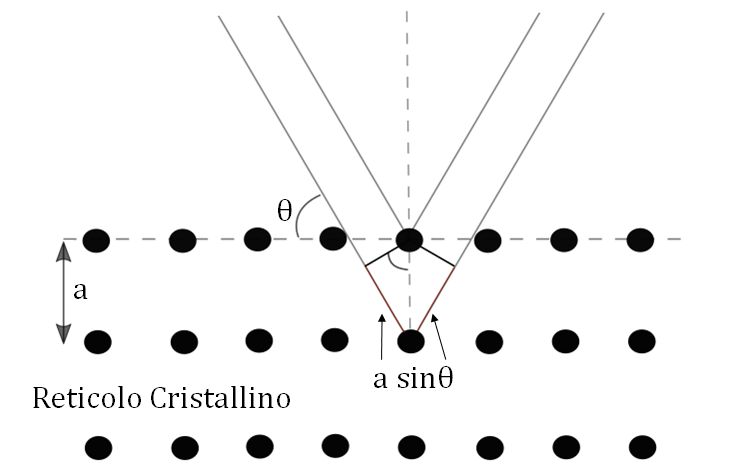
\includegraphics[width=.55\textwidth]{immagini/cap_1/fig_1_5.png}
		\end{center}
	\end{figure}
\newpage
La differenza di fase tra due onde diffuse  da piani adiacenti del reticolo cristallino è data da:
	\begin{equation}
		\delta = k \Delta x = \frac{2 \pi}{\lambda} 2a \sin \theta.
	\end{equation}
Si osserverà allora interferenza costruttiva quando questa differenza è pari ad un multiplo intero di $2 \pi$: $k \Delta x = 2 \pi n$, ossia:
	\begin{equation}
		\tcboxmath[sharp corners=downhill ,colback=white,colframe=red!75!black]{
			2a \sin \theta = n\lambda.
			}
	\end{equation}
Una figura di diffrazione, i cui massimi si presentano in corrispondenza degli angoli definiti dalla precedente equazione, venne effettivamente osservata negli esperimenti. la lunghezza d'onda, associata ad elettroni di impulso $p$, risultò inoltre in accordo con la formula di De Broglie. Questa osservazione rappresentò pertanto un passo fondamentale nella formulazione della \textbf{meccanica ondulatoria}.
\section{L'esperimento di Rutherford e gli spettri atomici}
Nel 1897 Thomson scopre gli elettroni. Nel 1908 \textbf{Rutherford} effettuò un \textbf{esperimento per studiare la struttura atomica.} L'esperimento consisteva nel bombardare sottili fogli di metallo con particelle $\alpha$, prodotte dal decadimento radioattivo. Il risultato inatteso fu che una significativa frazione di particelle $\alpha$ veniva deviata a grandi angoli di diffusione.\\

Il risultato dell'esperimento di Rutherford era inconsistente con le aspettative basate sul \textbf{modello di Thomson} dell'atomo. In questo modello si ipotizzavano gli elettroni immersi in una distribuzione di carica positiva, la cui estensione determina le dimensioni dell'atomo. Tuttavia gli elettroni non deviano le particelle $\alpha$, avendo una massa circa $10^4$ volte più piccola. Pertanto la sorgente che diffonde le particelle $\alpha$ deve essere la carica positiva, e grandi angoli di diffusione implicano che il potenziale sulla superficie della distribuzione di carica è grande. Questo a sua volta implica che la carica positiva è confinata in una regione di spazio molto più piccola dell'atomo.\\

\textbf{Rutherford} propose un \textbf{nuovo modello} in grado di spiegare i dati. In questo modello tutta la carica positiva (e quasi tua la massa) è concentrata in una piccola regione al centro dell'atomo. Questo nucleo d carica positiva attrae gli elettroni, carichi negativamente e, poiché la legge di forza ha un andamento $1/r^2$, \textbf{gli elettroni si muovono in orbite circolari od ellittiche attorno a nucleo.}\\

Sebbene in grado di spiegare i dati sperimentali relativi alla diffusione delle particelle $\alpha$, il modello di Rutherford presentava \textbf{due insuperabili difficoltà:}
	\begin{itemize}
		\item \textbf{Manca un meccanismo per stabilizzare gli atomi}: gli elettroni in orbite circolari od ellittiche sono costantemente accelerati e, secondo la teoria elettrodinamica classica, dovrebbero irradiare. La continua perdita di energia condurrebbe, in un tempo molto breve (dell'ordine di $10^{-10}$ s) al collasso dell'atomo con gli elettroni che cadono sopra il nucleo;
		\item Il modello non è in grado di spiegare gli \textbf{spettri atomici}, che si osservavano avere la struttura
			\begin{equation}
				\tcboxmath[sharp corners=downhill ,colback=white,colframe=red!75!black]{
					\frac{1}{\lambda} = cost. \left( \frac{1}{n_1 ^2}-\frac{1}{n_2 ^2} \right),
					}
			\end{equation}
		dove $n_1$ ed $n_2$ sono numeri interi.\\
\end{itemize}

Queste evidenti difficoltà tecniche nell'interpretazione dei risultati sperimentali relativi alla struttura atomica giocarono un ruolo fondamentale nello sviluppo della teoria quantistica.
\section{Modello di Bohr dell'atomo di idrogeno (1913)}
\textbf{Tre ipotesi:}
	\begin{itemize}
	\item l'elettrone ruota attorno al nucleo su orbite stabili (senza emettere radiazione);
	\item le sole orbite consentite sono quelle per le quali il momento angolare risulta un multiplo intero di $\hbar$\footnote{poiché $p= mv =\hbar/\lambda$ (De Broglie, \textbf{1923}) l'equazione (\ref{eq:cap1_4}) equivale a $2\pi r=n\lambda$.}:
		\begin{equation}
			L= mvr =n\hbar ;
		\label{eq:cap1_4}
		\end{equation}
	\item l'elettrone può effettuare transizioni discontinue tra due orbite consentite. Quando ciò accade viene emessa o assorbita radiazione di frequenza
	\begin{equation}
			\hbar \omega = E-E' ,
		\label{eq:cap1_5}
		\end{equation}
dove $E-E'$ è la variazione di energia dell'elettrone tra le due orbite.\\
	\end{itemize}
	
\textbf{Conseguenze}:
La stabilità di un'orbita è determinata dall'equilibrio tra la forza coulombiana e la forza centrifuga\footnote{Forza centrifuga: $F= m\omega ^2 r = mv^2 /r$.}
	\begin{equation}
	\frac{e^2}{r^2}=\frac{mv^2}{r} .
	\end{equation}	
Questa condizione, unita alla (\ref{eq:cap1_4}), fornisce
	\begin{equation}
		\begin{cases}
		mv^2 r= e^2 \\
		mvr =n\hbar		
		\end{cases}
		\Rightarrow v=\frac{e^2}{n\hbar}, \quad r=\frac{n\hbar}{mv}=\frac{n^2 \hbar ^2}{me^2} .
	\end{equation}
Dunque
	\begin{equation}
	r=n^2 \frac{\hbar ^2}{me^2}= n^2 a_0 \qquad \left[\textrm{in MQ}\ \left\langle\frac{1}{r}\right\rangle = \frac{1}{n^2 a_0}\right],
	\end{equation}
		\begin{equation}
	\frac{v}{c}= \frac{1}{n}\frac{e^2}{\hbar c}=\frac{\alpha}{n} \qquad \left[\textrm{in MQ}\ \left\langle\frac{v^2}{c^2}\right\rangle = \frac{\alpha ^2}{n^2}\right].
	\end{equation}
Calcoliamo l'energia delle orbite:
	\begin{equation}
		\frac{p^2}{2m}= \frac{mv^2}{2} =\frac{me^4}{2n^2 \hbar ^2} =\frac{mc^2 \alpha ^2}{2n^2},
		\label{eq:cap1_6}
	\end{equation}
	\begin{equation}
		\frac{e^2}{r}= \frac{me^4}{n^2 \hbar^2} =\frac{mc^2 \alpha ^2}{n^2},
		\label{eq:cap1_7}
	\end{equation}
da cui\footnote{In meccanica quantistica i risultati ottenuti per le equazioni (\ref{eq:cap1_6}) e (\ref{eq:cap1_7}) valgono per i valori medi, rispettivamente, di $T$ e $V$.}
	\begin{equation}
		\tcboxmath[sharp corners=downhill ,colback=white,colframe=red!75!black]{
			E=\frac{p^2}{2m}-\frac{e^2}{r}=-\frac{mc^2\alpha ^2}{2n^2}. }
	\end{equation}
Le righe di emissione e assorbimento dell'atomo hanno pertanto frequenze della forma:
	\begin{equation}
		\tcboxmath[sharp corners=downhill ,colback=white,colframe=red!75!black]{
			\hbar \omega = E-E' =\frac{mc^s \alpha ^2}{2}\left(\frac{1}{n^{\prime \, 2}} - \frac{1}{n^2}\right).
			}
	\end{equation}
